\documentclass[modern, letterpaper]{aastex61}
% \documentclass[twocolumn]{aastex61}

% TODO:
% -

% style notes
% -----------
% - Use the Makefile; don't be typing ``pdflatex'' or some bullshit.
% - Line break between sentences to make the git diffs readable.
% - Use \, as a multiply operator.
% - Reserve () for function arguments; use [] or {} for outer shit.
% - Use \sectionname not Section, \figname not Figure, \documentname not Article

\include{gitstuff}
% Load common packages

\usepackage{amsmath}
\usepackage{amsfonts}
\usepackage{amssymb}
\usepackage{booktabs}

\usepackage{graphicx}
\usepackage{color}

\usepackage{hyperref}
\definecolor{linkcolor}{rgb}{0.02,0.35,0.55}
\definecolor{citecolor}{rgb}{0.4,0.4,0.4}
\hypersetup{colorlinks=true,linkcolor=linkcolor,citecolor=citecolor,
            filecolor=linkcolor,urlcolor=linkcolor}
\hypersetup{pageanchor=false}

\newcommand{\documentname}{\textsl{Article}}
\newcommand{\sectionname}{Section}
\newcommand{\figname}{Figure}
\newcommand{\eqname}{Equation}
\newcommand{\tblname}{Table}

% Packages / projects / programming
\newcommand{\package}[1]{\texttt{#1}}
\newcommand{\acronym}[1]{{\small{#1}}}
\newcommand{\github}{\package{GitHub}}
\newcommand{\python}{\package{Python}}

% Missions
\newcommand{\project}[1]{\textsl{#1}}

% For referee
\newcommand{\changes}[1]{{\color{red} #1}}

% Stats / probability
\newcommand{\given}{\,|\,}
\newcommand{\norm}{\mathcal{N}}

% Maths
\newcommand{\dd}{\mathrm{d}}
\newcommand{\transpose}[1]{{#1}^{\!\mathsf{T}}}
\newcommand{\inverse}[1]{{#1}^{-1}}
\newcommand{\argmin}{\operatornamewithlimits{argmin}}
\newcommand{\argmax}{\operatornamewithlimits{argmax}}
\newcommand{\mean}[1]{\left< #1 \right>}
\renewcommand{\vec}[1]{\bs{#1}}
\newcommand{\mat}[1]{\mathbf{#1}}

% Unit shortcuts
\newcommand{\msun}{\ensuremath{\mathrm{M}_\odot}}
\newcommand{\kms}{\ensuremath{\mathrm{km}~\mathrm{s}^{-1}}}
\newcommand{\au}{\ensuremath{\mathrm{au}}}
\newcommand{\pc}{\ensuremath{\mathrm{pc}}}
\newcommand{\kpc}{\ensuremath{\mathrm{kpc}}}
\newcommand{\kmskpc}{\ensuremath{\mathrm{km}~\mathrm{s}^{-1}~\mathrm{kpc}^{-1}}}

% Misc.
\newcommand{\bs}[1]{\boldsymbol{#1}}

% Astronomy
\newcommand{\DM}{{\rm DM}}
\newcommand{\feh}{\ensuremath{{[{\rm Fe}/{\rm H}]}}}
\newcommand{\df}{\acronym{DF}}

% TO DO
\newcommand{\todo}[1]{{\color{red} TODO: #1}}

\graphicspath{{figures/}}

% Project-specific
\newcommand{\gaia}{\project{Gaia}}
\newcommand{\DR}[1]{\acronym{DR}1}
\newcommand{\tgas}{\acronym{TGAS}}
\newcommand{\lbfgsb}{\texttt{L-BFGS-B}}
\newcommand{\Ha}{\ensuremath{{\rm H}\alpha}}

\begin{document}

\title{Co-moving stars in \textsl{Gaia DR1}:
       a catalog of genuine comoving star pairs from low-resolution
       spectroscopic follow-up}

\author{Adrian~M.~Price-Whelan}
\affiliation{Department of Astrophysical Sciences,
             Princeton University, Princeton, NJ 08544, USA}
\affiliation{To whom correspondence should be addressed:
             \texttt{adrn@astro.princeton.edu}}

\author{Semyeong~Oh}
\affiliation{Department of Astrophysical Sciences,
             Princeton University, Princeton, NJ 08544, USA}

\author{David~N.~Spergel}
\affiliation{Flatiron Institute,
             Simons Foundation,
             162 Fifth Avenue,
             New York, NY 10010, USA}
\affiliation{Department of Astrophysical Sciences,
             Princeton University, Princeton, NJ 08544, USA}

% \author{Melissa~Ness}
% \affiliation{todo}

% \author{David~W.~Hogg}
% \affiliation{todo}

\begin{abstract}
% Context
Widely-separated, co-eval stars are [...] for studying the chemical homogeneity
of birth, calibrating stellar atmosphere models across a range of [..], and for
modeling the Galactic tidal field.
Previous work using Hipparcos + literature RVs -> a few hundred genuine pairs
out to 8 pc.
% Aims
Identified candidate pairs using the Tycho-Gaia Astrometric Solution catalog,
Gaia DR1.
Want to identify genuinely dynamically associated pairs for future
high-resolution follow-up
% Methods
Low-resolution spectrograph to measure relative radial velocities to identify
genuine pairs.
% Results
Of the XX pairs observed, we find YY ...
% Conclusions
Gaia DR2 -> how many do we expect?
\end{abstract}

\keywords{
    TODO
}

\section{Introduction}\label{sec:introduction}

Outline:
- Stars form in clusters, chemically homogeneous at some level
- Clusters generally disrupt slowly through a process that preserves initial
  clustering in conserved quantities but destroys phase coherence
- Most significant process is probably tidal heating
- Dissolved clusters are therefore useful dynamical tracers of mass distribution
- In Galactic halo, globular clusters
- In disk, hope is to use chemical signatures to connect stars, then can use
  dynamics to reconstruct birth clusters, infer mass distribution / evolution
- Clusters have advantage of many stars per cluster, but fewer clusters
- Wide binary stars are little potentiometers themselves - only N=2, but are far
  more numerous as a population
- Long-term goal is to study the separation distribution of wide-binaries as a
  function of age and Galactic orbit distribution (disk vs. halo)
    - Is there a separation truncation?
    - Can that be described just from Galactic tides, or need perturbers?
- Also useful for stellar models: should have same age, chemistry, but need to
  test this
    - Chemical homogeneity tested with few open clusters - wide binaries another
      test
    - Need sample of confirmed widely-separated binaries, follow-up to get
      detailed abundances
    - Need way to verify that widely separated stars are physically associated,
      via kinematics
- Some bullshit about Gaia, TGAS, etc., released as a part of \gaia\ \DR{1}\

\cite{Gaia-Collaboration:2016,Gaia-Collaboration:2016a}

Most stars form in clusters with small dispersions in position, velocity, and
(likely) small initial spreads in chemical abundances.
Once a given cluster is visibly dispersing or fully dispersed, the former member
stars retain chemical and kinematic signatures of their birth cluster

comoving not wide binary (don't know if they are bound)

, though
the kinematic mapping is non-trivial because of phase-mixing.

become
useful

Widely-separated comoving stars are expected to form from the dissolution of
birth star clusters


\section{Data}\label{sec:data}

\subsection{Sample selection}\label{sec:sample}

In previous work, we have identified a sample of high-confidence, candidate
comoving star pairs (\citealt{Oh:2017}) using only astrometric information from
the \tgas\ catalog (\citealt{tgas}).
These comoving pairs were selected using a cut on a marginalized likelihood
ratio computed for all nearly co-spatial pairs of stars.
For a full description of the selection method, see \citealt{Oh:2017}.
Briefly, likelihood 1, $L_1$, considers a model in which the full-space
velocities of each star in the pair are identical and sampled from a disk-like,
Sun-relative velocity distribution, and likelihood 2, $L_2$, considers a model
in which the full-space velocities of each star were drawn independently from
the same velocity distribution used above; the likelihood ratio is computed as
$L_1/L_2$.
After a parallax signal-to-noise ratio (SNR) cut ($\pi/\sigma_\pi > 8$), we
compute the likelihood ratio for all stars within $10~\pc$ of each target star
from the \tgas\ catalog.
The likelihoods appropriately take into account the reported covariances and
uncertainties between the astrometric measurements in the \tgas\ catalog and
naturally handle geometric or projection effects in comparing spherical
velocity components for star pairs separated by large angles on the sky.
After applying a conservative cut on the likelihood ratio motivated by
computing the same likelihood ratio for random pairings of stars, we find
13,058 comoving star pairs with physical separations between $10^3~\au$ and
$10~\pc$.
Of these pairs, there are 10,606 unique sources, implying that a significant
fraction of the identified pairs are members of larger groups.
$\approx$4,000 of the pairs are mutually exclusive, i.e. neither member is
paired with other stars.

To select candidate pairs for follow-up spectroscopic observations, we only
consider mutually exclusive star pairs within $200~\pc$ in Heliocentric
distance; with the SNR cut used above and given the limitations of the \tgas\
catalog itself, \tgas\ is $\approx$90\% complete to $200~\pc$
(\citealt{Bovy:2017}).
From this source target list, we randomly observed targets with airmass $\sec z
< 1.5$.

\todo{color-magnitude diagram of all stars observed, color our targets
different from the calibration targets}
\figurename~\ref{fig:sample-cmd} shows a color-magnitude diagram of all targets
observed in this observing run (markers) plotted over the density of all \tgas\
stars within $200~\pc$.

\begin{figure}[htbp]
  \begin{center}
    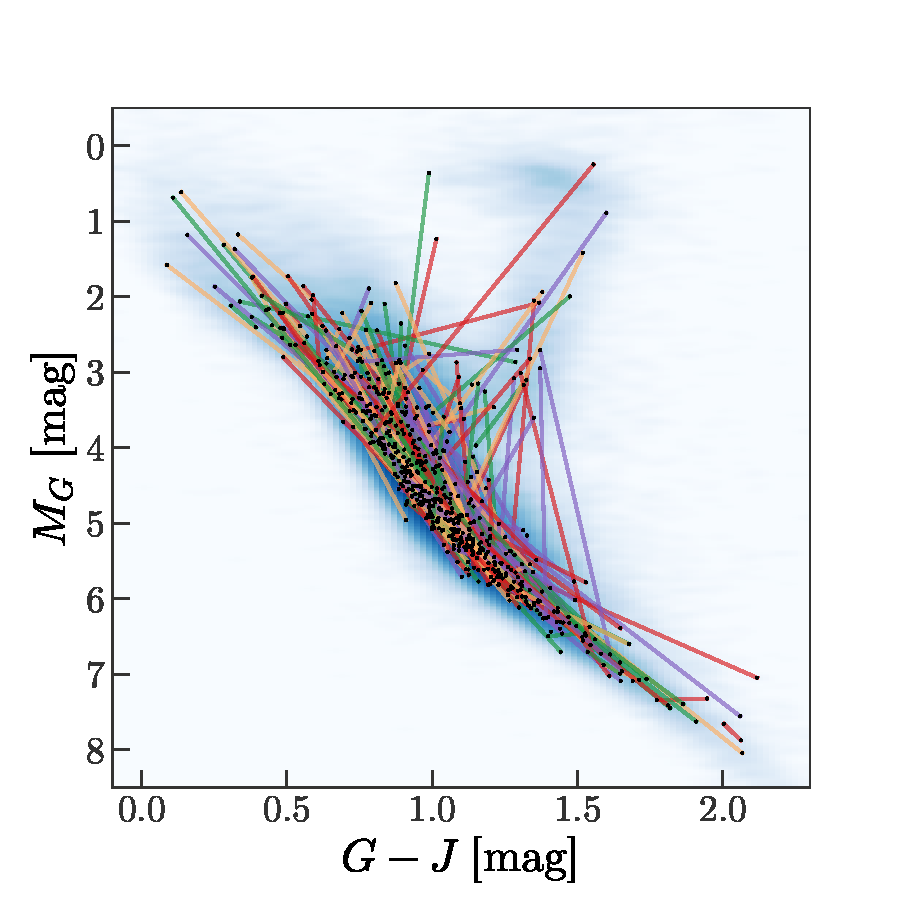
\includegraphics[width=\linewidth]{sample_cmd.pdf}
  \end{center}
  \caption{%
    Color-magnitude diagram for all \tgas\ sources within $200~\pc$ (background
    blue histogram) and all comoving star pair members observed in this
    follow-up effort (black points); colored lines connect candidate comoving
    star pairs.
    2MASS $J$-band magnitudes are obtained from the Gaia science
    archive.
    Apparent $G$-band magnitudes (\citealt{Carrasco:2016}) are converted to
    absolute magnitude, $M_G$, using a Lutz-Kelker-corrected
    (\citealt{Lutz:1973}) distance estimate (see also \eqname~1 in
    \citealt{Oh:2017}).
    \label{fig:sample-cmd}}
\end{figure}

\subsection{Observations and data reduction}\label{sec:reduction}

Spectra were obtained using the \project{Modspec} spectrograph mounted on the
$2.4~{\rm m}$ Hiltner telescope at MDM
observatory\footnote{\url{http://mdm.kpno.noao.edu}} on Kitt Peak (Arizona).
\project{Modspec} was set up in long-slit mode with a 1'' slit, a $600~{\rm
line}~{\rm mm}^{-1}$ grating, and a $2048\times2048~{\rm pixel}$ SITe CCD
detector (``Echelle'').
Only the central 300 pixel columns were read out from the CCD, and pixel rows
$>1600$ (at the blue end) were later trimmed because of the poor quantum
efficiency of the CCD at wavelengths $\lesssim 3600~{\rm \AA}$.
The resolution and wavelength range were $\approx2~{\rm \AA}~{\rm pixel}^{-1}$
from $\approx 3600$--$7200~{\rm \AA}$.
At this resolution, to obtain high signal-to-noise spectra, most exposures were
between $30$--$120~{\rm s}$ (15th and 85th percentiles).
To maximize the number of observed pairs, we therefore chose to not take
comparison lamp spectra at each pointing, which adds an overhead of $\approx
90~{\rm s}$ per observation.
To determine rough nightly wavelength solutions, spectra were obtained using
Hg-Ne and Ne comparison lamps at the beginning and end of each night, and
atmospheric emission lines were used to correct the wavelength solution on a
per-object basis.

We observed a total of 765 unique sources over 5 nights from (UT) 2017-03-11 to
2017-03-15, corresponding to 321 unique star pairs and $\approx 120$
calibration targets.
The calibration targets have previously measured radial velocities and chemical
abundances, which will be used for validation of our reduction pipeline and in
future work to measure metallicities and stellar parameters for each observed
source using \project{The Cannon} (\citealt{Ness:TODO}).
The spectra were reduced and calibrated using a custom, publicly-available
pipeline written in \python,\footnote{Released along with the code used to
generate the figures in this document at
\url{https://github.com/adrn/GaiaPairsFollowup}.} described below.

For each source or comparison lamp observation, the two-dimensional image is
bias corrected, flat-field corrected, and trimmed using standard routines
implemented in \package{ccdproc} (\citealt{Craig:2015}).
For comparison lamp observations, the central 100 pixel columns are extracted
and summed along the spatial axis, weighted by the inverse-variances of each
pixel.
Source spectral traces were always placed in this region during observations,
and the curvature of the wavelength solution over this region is negligible.
For source observations, the 2D spectra are extracted to 1D using an empirical
estimate of the pixel-convolved line spread function (LSF): at each of 16 pixel
rows between indices 750 and 850 (i.e. around the effective center of the
dispersion axis), a model for the LSF is fit to the 1D trace.
The LSF is assumed to be a Voigt profile with parameters $A$, amplitude; $x_0$,
profile centroid; $\sigma_G$, Gaussian root-variance; $\gamma_L$, Lorentzian
half-width at half maximum, and the background is modeled using a linear
polynomial with parameters $\alpha_1$ and $\alpha_2$, the slope and intercept
at the profile centroid, respectively.
The maximum-likelihood LSF + background model parameters are estimated from
each pixel row using \lbfgsb\ optimization (\citealt{Zhu:1994}), implemented in
the \package{scipy} package.
From the 16 fits, the median profile width parameters, $\sigma_G$ and
$\gamma_L$, are then taken to be the LSF width parameters.
At each of 1600 rows in each source spectrum image, the LSF amplitude and
centroid, and background slope and intercept at line centroid are then fit using
the same procedure as above but with the width parameters fixed.
The LSF amplitudes are stored as the source fluxes, and the background model
intercepts are stored as the background (sky) fluxes.
Occasionally, nearby sources fall in the slit; these are masked by hand in the
2D images and do not bias the LSF extraction fits.

We start the wavelength calibration by interactively identifying the 12
strongest, least blended emission lines in one of the extracted 1D comparison
lamp spectra by comparing to \todo{NIST??}.
Once a rough mapping from pixel to wavelength is determined, we then fit for
the individual line centroids in each comparison lamp spectrum by extracting
small, 8 pixel-wide segments of spectrum around each identified emission line
and fitting a model for the line profile and background to each individually.
We use a pixel-convolved Gaussian profile for each emission line with
parameters: amplitude, $A$; centroid, $x_0$; and root-variance, $\sigma_G$.
We find that nearby blended or low-amplitude lines (i.e. part of the
``background'') sometimes bias the line centroid determination when using a
simple background model.
We therefore model the background flux around each comparison lamp emission
line using a constant offset + Gaussian process (GP).
For the GP model, we use a Mat\'ern 3/2 kernel function
(\citealt{Matern:1986,Rasmussen:2005}) parametrized by amplitude parameter
$\sigma_{3/2}$ and correlation scale $\rho_{3/2}$.
We use \package{celerite} (\citealt{Foreman-Mackey:2017}) to evaluate the full
likelihood for this model, and maximize the (log-)likelihood again using
\lbfgsb\ optimization.
We optimize over the logarithm of any scale parameters (i.e. $A$, $\sigma_G$,
$\sigma_{3/2}$, and $\rho_{3/2}$).
Once we determine the pixel centroids for all identified emission lines for a
given night's comparison lamp spectrum, we then fit an interpolating function
to the pixel-centroid, wavelength values for each emission line.

Typically, high-order standard polynomials or Chebyshev polynomials are used to
fit for the wavelength dispersion function.
We found that using such functions can lead to vastly incorrect wavelength
values near either end of the pixel grid where the polynomial function is
un- or weakly-constrained.
We instead use a combined linear polynomial + GP to model the wavelength
dispersion.
We again use a Mat\'ern 3/2 kernel, use \lbfgsb\ optimization, and convert any
scale parameter to log-space before maximizing the log-likelihood.
\figurename~\ref{fig:wavelength-GP} shows an example of the residuals from one
such fit; black points show the (pixel-centroid, wavelength) pairs with the
best-fit model subtracted.
The envelope around zero (shaded region, orange) shows the \todo{1$\sigma$ blah
blah GP...}
When the GP variance is large, the pixel-to-wavelength mapping is uncertain.
We therefore only use the pixel range from 250--1210, corresponding to a
wavelength range of $\approx 5500$--$7400~{\rm \AA}$; gray shaded region shows
the excluded pixel/wavelength ranges.

This wavelength calibration procedure produces a nightly model for the
nonlinear dispersion of wavelength as a function of pixel value for each
extracted 1D spectrum.
However, because of flexure in the spectrograph, each observation will have an
additional offset of, typically, $\approx 0.5$--$2~{\rm \AA}$, corresponding to
a significant velocity offset at \Ha\ of $\approx 25$--$100~\kms$.
\figurename~\ref{fig:sample-spectra} shows a random sample of 10
wavelength-calibrated source spectra of comoving star pair members normalized
to 1 at $\lambda = 5500~{\rm \AA}$ and shifted by index for visualization.
Suggested by the features in these 10 spectra, there is a mix of metallicities
and spectral types amongst the observed targets.
Note that the spectra are not flux-calibrated, as we only care about measuring
radial velocities from this sample.

\begin{figure}[htbp]
  \begin{center}
    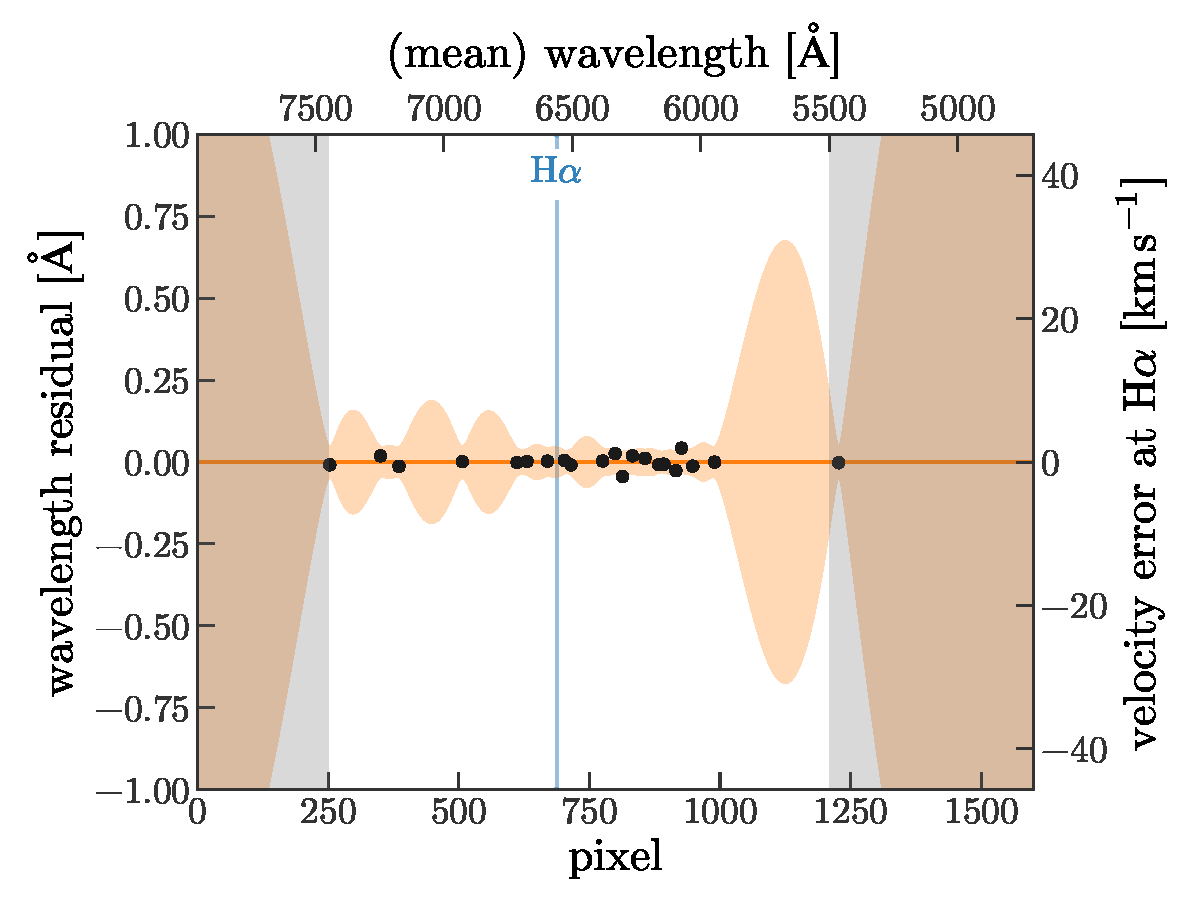
\includegraphics[width=\linewidth]{wavelength_gp.pdf}
  \end{center}
  \caption{%
    A visualization of the pixel-to-wavelength model determined from a single
    wavelength comparison lamp spectrum.
    Black markers show the fit pixel centroids for known Hg or Ne emission
    lines and the residual wavelength value between the linear + GP model and
    the true emission line centroid.
    The non-shaded region shows the section of spectrum where the comparison
    lamp spectrum has sufficient line density to determine the wavelength
    solution; shaded regions are masked from the resulting spectra.
    Orange envelope shows the root-variance of the Gaussian process component
    of the model, which can be interpreted as inherent uncertainties on the
    wavelength calibration as a result of the model flexibility.
    \label{fig:wavelength-GP}}
\end{figure}

\begin{figure}[htbp]
  \begin{center}
    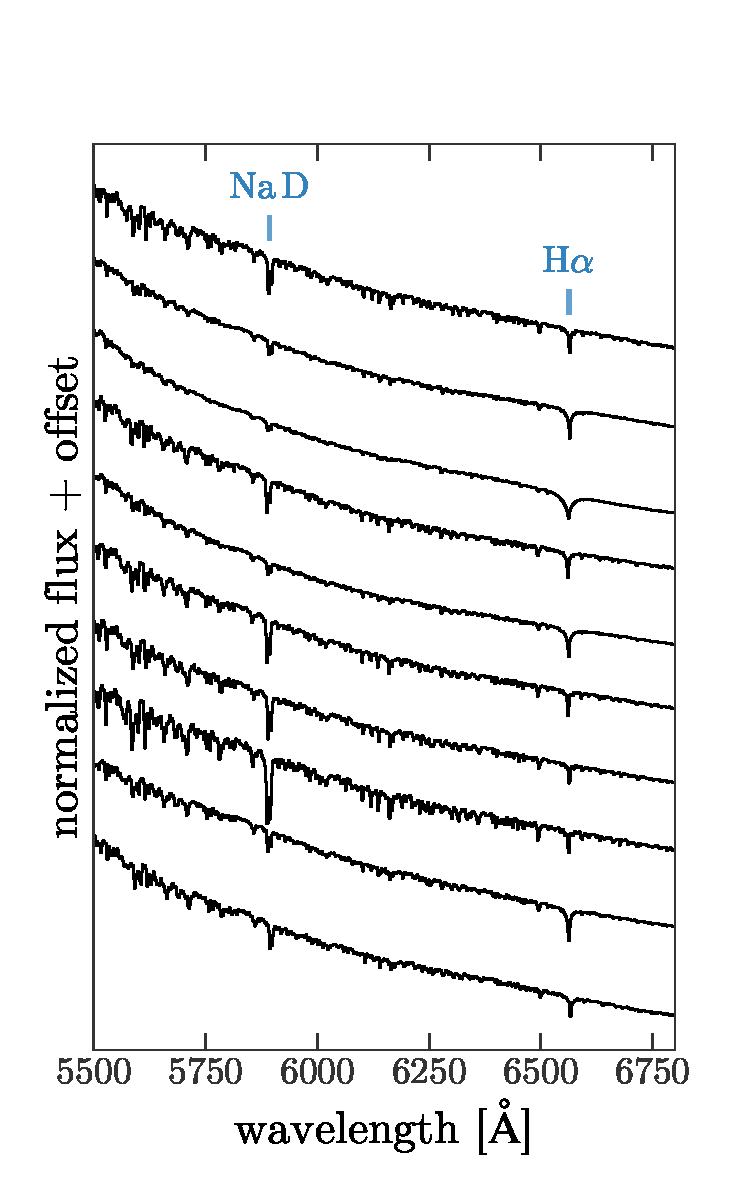
\includegraphics[width=0.9\linewidth]{sample_spectra.pdf}
  \end{center}
  \caption{%
    A section of 10 randomly selected target spectra from this work.
    Spectral fluxes are normalized to 1 at $\lambda = 5500~{\rm \AA}$ and the
    offsets are chosen to separate the spectra for visualization.
    The spectra are smoothed with a Gaussian filter with root-variance $\sigma
    = 2~{\rm \AA}$.
    \label{fig:sample-spectra}}
\end{figure}

As mentioned, comparison lamp spectra were not obtained at each telescope
pointing.
The absolute wavelength solution at each pointing can therefore be shifted
(in pixels) relative to the nightly comparison lamp spectrum because of flexure
in the instrument.
We have found that this offset depends primarily on the hour angle of the
observation, likely because of the physical orientation of the spectrograph and
CCD as mounted on the telescope.
To correct each source spectrum for this offset, we measure the centroids of
the two prominent [OI] sky emission lines near $5577~{\rm \AA}$ and $6300~{\rm
\AA}$ in the corresponding background spectrum derived from the spectral
extraction (described above).
We use a pixel-convolved Voigt profile as the emission line model (same
parameters as above) and a Gaussian process with a Mat\'ern 3/2 kernel function
for the background spectrum (same parameters as above).
We again use \lbfgsb\ optimization and convert any scale parameter to log-space
before maximizing the log-likelihood of this model to derive the line centroid
in wavelength units.
We compute wavelength offsets from true (air) values of the line centroids,
$5577.3387~{\rm \AA}$ and $6300.304~{\rm \AA}$ respectively,\footnote{\url{http:
//physics.nist.gov/PhysRefData/ASD/lines_form.html}} then convert these
wavelength offsets to pixel offsets.
We take the mean of the pixel offsets and apply the derived shift to the source
spectrum before re-computing the wavelength grid using the nightly wavelength
solution \todo{is this sensible?}.
When one or both of the two sky lines is not present or the centroid fit fails,
the spectrum \todo{flagged in some way, can have large absolute velocity
systematic error.}

To derive radial velocities for each source, we then measure the (wavelength)
line centroid of \Ha\ in each corrected spectrum.
We model the absorption line using a pixel-convolved Voigt profile and use a
linear model + a Gaussian process for the background model.
We now use \lbfgsb\ optimization and the resulting maximum-likelihood parameters
to initialize a Markov Chain Monte Carlo (MCMC) sampling of the posterior
probability distribution (pdf) over the 8 parameters: $\ln |A|$, $x_0$,
$\ln\sigma_G$, $\ln\gamma_L$, $\alpha_1$, $\alpha_2$, $\ln\sigma_{3/2}$, and
$\ln\rho_{3/2}$ where the linear background model is defined as $f(\lambda) =
\alpha_1 + \alpha_2\,\lambda$.
The linear amplitude, $A$, is assumed to be negative (i.e. \Ha\ is assumed to be
an absorption feature) and is computed from the corresponding parameter as $A =
-\exp(\ln |A|)$.
We use uniform priors on all parameters except $\ln\rho_{3/2}$, for which we use
a Gaussian; prior parameters are specified in \tablename~\ref{tbl:prior-bounds}.
We use \package{emcee} (\citealt{Foreman-Mackey:2013}) with 64 walkers to
generate samples from the posterior pdf.
We initially run the sampler for 128 steps from the maximum likelihood parameter
values, then resample walker positions in a small ball around the median final
walker positions and run again for 512 steps; together, these two steps
constitute our burn-in phase.
From the final walker positions after burn-in, we run again for 1024 steps and
store these as our primary posterior samples.
\figurename~\ref{fig:Halpha-mcmc} shows


With the resulting posterior samples, we compute the median and median absolute
deviation (MAD) of the marginal distribution over line centroid, $x_0$.
We use the MAD to estimate the standard deviation ($\sigma \approx 1.5\times{\rm
MAD}$, assuming the samples are Gaussian distributed) of the samples and find
that the typical velocity \emph{precision} from measuring the centroid of \Ha\ is between $2$--$10~\kms$ \todo{double check numbers}.

\begin{table}[ht]
  \begin{center}
    \begin{tabular}{ c | c }
      \toprule
        Parameter & Prior \\\toprule
        $\ln A$ & $\mathcal{U}(2, 16)$\\
        $x_0$ & $\mathcal{U}(6547, 6579)$\\
        $\ln\sigma_G$ & $\mathcal{U}(-4, 2)$\\
        $\ln\gamma_L$ & $\mathcal{U}(-4, 2)$\\
        $\alpha_1$ & $\mathcal{U}(0, 10^{16})$\\
        $\alpha_2$ & $\mathcal{U}(-10^8, 10^8)$\\
        $\ln\sigma_{3/2}$ & $\mathcal{U}(-8, 8)$\\
        $\ln\rho_{3/2}$ & $\mathcal{N}(1, 1)$\\
      \bottomrule
    \end{tabular}
    \caption{
      Priors used for \Ha\ line profile model parameters.
      $\mathcal{U}(a, b)$ indicates a uniform prior between $a$ and $b$ and
      $\mathcal{N}(\mu, \sigma^2)$ indicates a normal distribution with mean
      $\mu$ and variance $\sigma^2$.
      Wavelength units are all angstroms.
      \label{tbl:prior-bounds}
    }
  \end{center}
\end{table}

\begin{figure}[htbp]
  \begin{center}
    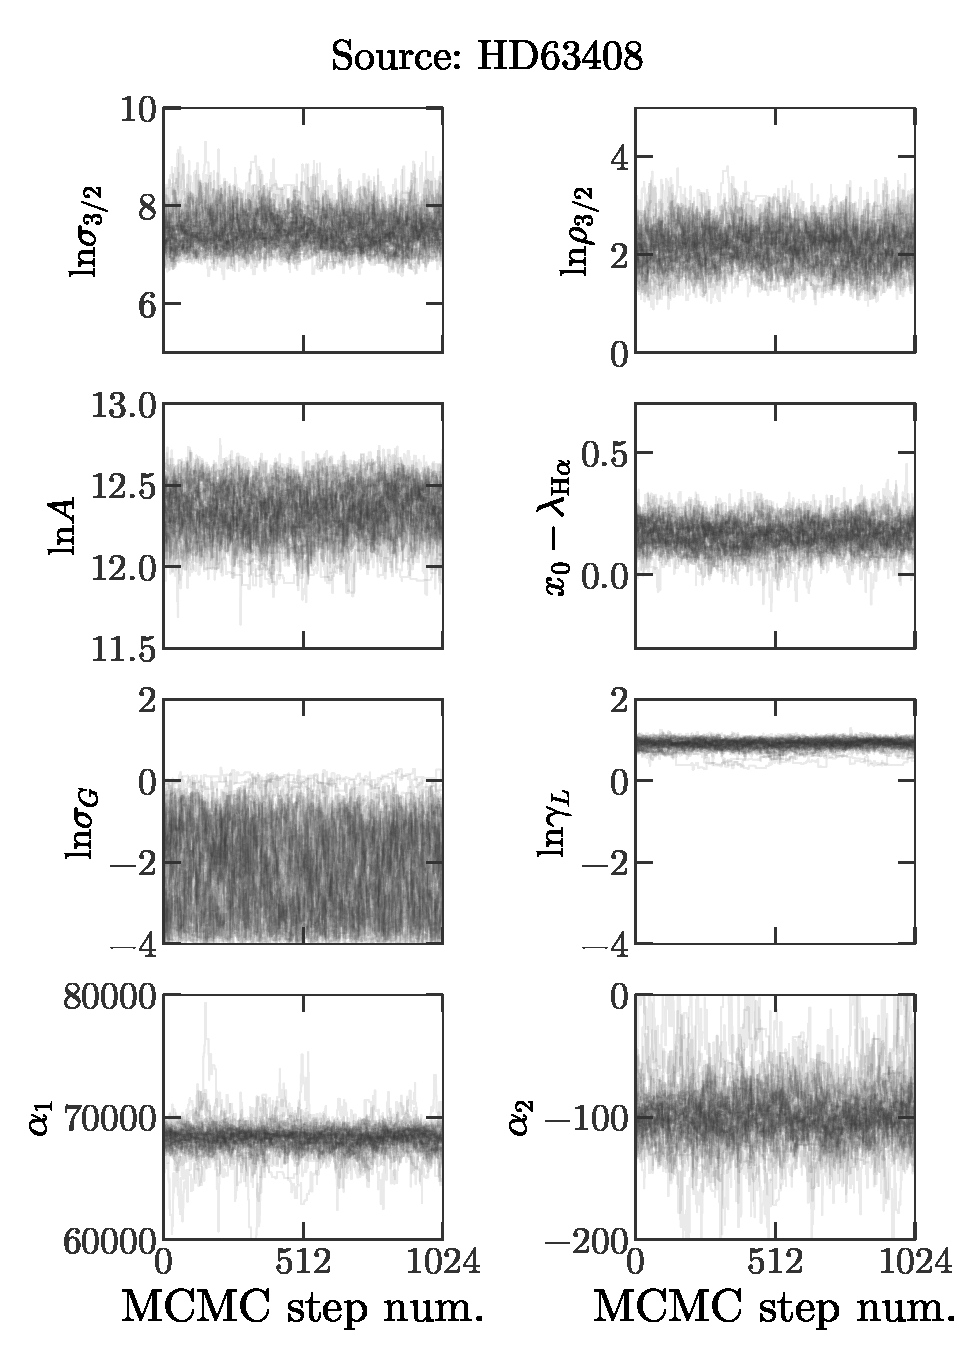
\includegraphics[width=\linewidth]{mcmc_trace.pdf}
  \end{center}
  \caption{%
    \todo{Some summary plots about the MCMC fits...}
    \label{fig:Halpha-mcmc}}
\end{figure}

\begin{figure}[htbp]
  \begin{center}
    \includegraphics[width=\linewidth]{example_fit.pdf}
  \end{center}
  \caption{%
    \todo{More MCMC bullshit.}
    \label{fig:compare-previous}}
\end{figure}

Several of our targets and all of our calibration targets have previously
measured radial velocities.
We can therefore estimate our absolute velocity accuracy by comparing our
derived radial velocities with previous measurements.
\todo{Explain how we get previous measurements - Simbad or explicit catalogs?}
\figurename~\ref{fig:compare-previous} shows the distribution of differences
between our measurements and literature values \todo{uncertainties??}.

TODO: Comparing repeat visits on subsequent nights, absolute errors ~20 km/s
- How many of our targets already have measurements in Simbad?

% \begin{figure}[htbp]
%   \begin{center}
%     \includegraphics[width=\linewidth]{example_fit.pdf}
%   \end{center}
%   \caption{%
%     \todo{Plot showing my RV's vs. previously measured.}
%     \label{fig:compare-previous}}
% \end{figure}

% See: http://iopscience.iop.org/article/10.1088/0004-6256/146/6/161/pdf for an example

\section{Results}

\subsection{Catalog ...}\label{sec:}

TODO: 10 overlap with Shaya and Olling

TODO: Do I want to do isochrone fitting for all of them?

\subsection{Physical properties of genuine comoving pairs}\label{sec:}

TODO: Plot of magnitude of 3d velocity difference vs. 3d separation (inferred).

TODO: separation distribution - combine with Shaya and Olling sample!

TODO: distribution of orbital poles in Galactic coordinates

\subsection{Galactic orbits of the co-moving pairs}\label{sec:}

TODO: Orbits of true pairs in the Galaxy, any halo or thick-disk?

\section{Discussion}

Abundances!

\section{Conclusions }

\acknowledgements
John Brewer (Yale),
Jason Curtis (Columbia),
James Davenport (WWU) for PyDIS,
David W. Hogg (NYU),
Melissa Ness (MPIA)

This work is based on observations obtained at the MDM Observatory, operated by
Dartmouth College, Columbia University, Ohio State University, Ohio University,
and the University of Michigan.
This work has made use of data from the European Space Agency (ESA)
mission {\it Gaia} (\url{https://www.cosmos.esa.int/gaia}), processed by
the {\it Gaia} Data Processing and Analysis Consortium (DPAC,
\url{https://www.cosmos.esa.int/web/gaia/dpac/consortium}). Funding
for the DPAC has been provided by national institutions, in particular
the institutions participating in the {\it Gaia} Multilateral Agreement.
% The authors are pleased to acknowledge that the work reported on in this
% paper was substantially performed at the TIGRESS high performance computer
% center at Princeton University which is jointly supported by the Princeton
% Institute for Computational Science and Engineering and the Princeton
% University Office of Information Technology's Research Computing department.

\software{
The code used in this project is available from
\url{https://github.com/adrn/GaiaPairsFollowup} under the MIT open-source
software license.
This research utilized the following open-source \python\ packages:
    \package{Astropy} (\citealt{Astropy-Collaboration:2013}),
    \package{astroquery} (\citealt{Ginsburg:2016}),
    \package{ccdproc} (\citealt{Craig:2015}),
    \package{celerite} (\citealt{Foreman-Mackey:2017}),
    \package{emcee} (\citealt{Foreman-Mackey:2013ascl}),
    \package{IPython} (\citealt{Perez:2007}),
    \package{matplotlib} (\citealt{Hunter:2007}),
    \package{numpy} (\citealt{Van-der-Walt:2011}),
    \package{scipy} (\url{https://www.scipy.org/}),
    \package{sqlalchemy} (\url{https://www.sqlalchemy.org/})
This work additionally used the Gaia science archive
(\url{https://gea.esac.esa.int/archive/}).
}

\facility{MDM: Hiltner (Modspec)}

\bibliographystyle{aasjournal}
\bibliography{refs}

\end{document}
